\section{Path-View: Neural Path Features and Information Flow}\label{sec:pathgate}
\textbf{Notation:} We consider fully connected deep networks with $d$ layers, and $w$ hidden units per layer, which accepts an input $x\in\R^{d_{in}}$, and produces an output $\hat{y}_{\Theta}\in \R$ where $\Theta\in\R^{d_{net}}$ ($d_{net}=w^2(d-2)+w(d_{in}+1)$). We denote by $\Theta(l,i,j)$ the weight connecting the $i^{th}$ hidden unit of layer $l-1$ to the $j^{th}$ hidden unit of layer $l$, and we use $G_{x,\Theta}(l,i)$ be the gating value ($0/1$) of the $i^{th}$ hidden unit in layer $l$ for an input $x\in \R^{d_{in}}$.\\
\textbf{Paths:}  We have a total of $P=d_{in}w^{(d-1)}$ paths. Let us say that an enumeration of the paths is given by $[P]=\{1,\ldots,P\}$. Let $\I_{l}\colon [P]\ra [w],l=0,\ldots,d-1$ provide the index of the hidden unit through which a path $p$ passes in layer $l$ (with the convention that $\I_d(p)=1,\forall p\in [P]$). The activity of a path $p$ for an input $x\in \R^{d_{in}}$ by $A_{\Theta}(x,p)\stackrel{def}{=}\Pi_{l=1}^{d-1} G_{x,\Theta}(l,\I_l(p))$.\\
We define $\phi_{x,\Theta}\stackrel{def}=(x_s(\I_0(p))A_{\Theta}(x_s,p) ,p\in[P])\in\R^P$ to be the \textbf{neural path feature} (NPF) of an input $x\in\R^{d_{in}}$, where, for a path $p$, $\I_0(p)$ is the input node at which the path starts, and $A_{\Theta}(x_s,p)$ is its activity. %By arranging the NPF of the $n$ input examples in a matrix $\Phi_t=(\phi_{x_s,\G_t},s\in[n])\in\R^{P\times n}$, we can express 
We define $v_{\Theta}\stackrel{def}=(\Pi_{l=1}^d \Theta(l,\I_{l-1}(p),\I_l(p)),p\in[P])\in\R^P$ to be the \textbf{neural path value} (NPV). The zeroth and first-order terms of a DNN can be written as:
\begin{align}
\label{eq:zero}\text{(Zeroth-Order)}\quad: \quad \hat{y}_{\Theta}(x)&=\ip{\phi_{x,\Theta},v_{\Theta}}=\sum_{p\in [P]}x(\I(p))A_{\Theta}(x,p)v_{\Theta}(p)\\
\label{eq:first}\text{(First-Order)}\quad: \quad \partial \hat{y}_{\Theta}(x)&=\underbrace{\ip{\phi_{x,\Theta},\partial v_t}}_{\text{value gradient}}+ \underbrace{\ip{\partial\phi_{x,\Theta},v_{\Theta}}}_{\text{feature gradient}}\\&=\sum_{p\in [P]}x(\I(p)) A_{\Theta}(x,p) \partial(v_{\Theta}(p))+\sum_{p\in [P]}x(\I(p)) \partial(A_{\Theta}(x,p)) v_{\Theta}(p)\nn
\end{align}
\textbf{Gating:} In what follows, we consider two kinds of gates namely, i) hard gates, taking values in $\{0,1\}$, and ii) soft gates, taking values in $(0,1)$. For a pre-activation input $q\in\R$, the  hard and soft gates are given by $G(q)=\mathbbm{1}_{\{\q>0\}}$ and $G(q)=\frac{1}{1+\exp(-\beta q)}$, where $\beta>0$ is a positive constant. Using the hard and soft gates, we can specify the ReLU and `soft-ReLU' activations as $\chi(q)=q\cdot\mathbbm{1}_{\{q>0\}}$ and $\chi(q)=q\cdot\left(\frac{1}{1+\exp(-\beta q)}\right)$.
\subsection{Information Flow: Zeroth-Order}
$1.$ \textbf{Representational Power Vs Scale Invariance:} The ability of DNNs to fit data has been demonstrated in the past. \cite{ben} showed that DNNs can fit even random labels, and random pixels of standard datasets such as MNIST. However, we note that, for DNNs with ReLU, with no bias parameters, a dataset with $n=2$ points namely $(x,1)$ and $(x/2,-1)$ for some $x\in \R^{d_{in}}$ cannot be memorised. The reason is that the gating values are the same for both $x$ and $x/2$ (for that matter any positive scaling of $x$), and hence $\phi_{x/2,\Theta}= \phi_{x,\Theta}/2$, and thus it not possible to fit arbitrary values for $\hat{y}_t(x/2)$ and $\hat{y}_t(x)$, since $\hat{y}_t(x/2)= \hat{y}_t(x)/2$. Cartoons $(a)$ and $(b)$ in \Cref{fig:cartoon} illustrate this scale invariance for inputs $x=(1,-1,2)\in\R^3$ and $x/2=(0.5,-0.5,1)\in\R^3$:  when compared to $(a)$, pre-activation values and output of $(b)$ are scaled down by a factor $2$, and the gating values of $(a)$ and $(b)$ are identical.\\
$2.$ \textbf{Translation Invariance:} Consider a convolution network using $l$ layers of circular convolutions\footnote{Here, instead of zero-padding in the corners, we follow the convention that index $d_{in}+k$ will be interpreted as $k$, for $k>0$, and $-k$ will be interpreted as $d_{in}-k$.} with filter size $k'<d_{in}$ and unit stride, and let $x^l(i)$ be the output of the $i^{th}$ channel after either $\max$-/global-average-pooling. Looking at the third and fourth (from left) illustrations in \Cref{fig:cartoon}, it is easy to check the translation invariance property: each of the red, blue, green lines have the same path values due to weight sharing in the convolutional layers, this leads to a circular symmetry in the path values, due to which, a translation in the input will cause all the internal variable to translate, and final invariance results from the invariance of the $\max$/average operation.\\
$3.$ \textbf{Active Sub-Network:} For each input example, a set of gates are \emph{on} in each layer, and this gives rise to the sub-network of active paths for that input. This active sub-network can be said to hold the memory for a given input (see cartoon $(b)$ in \Cref{fig:cartoon}).
\begin{figure*}[t]
%\begin{minipage}{0.78\columnwidth}
\resizebox{\columnwidth}{!}{
\begin{tabular}{ccc}
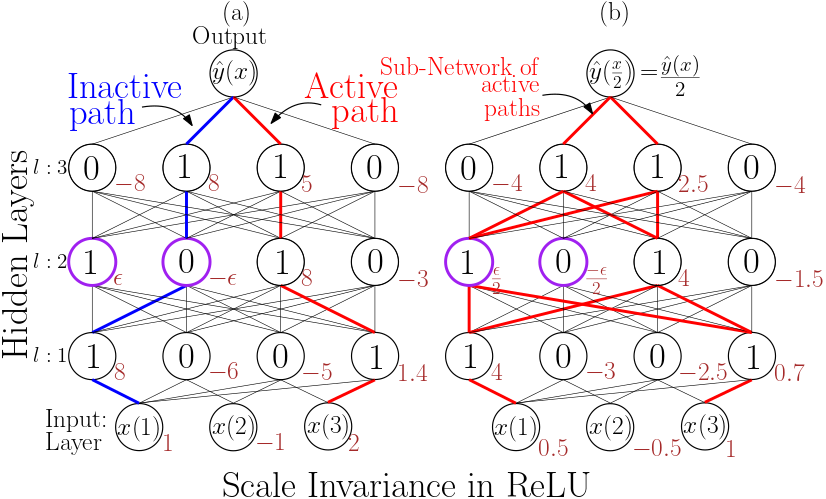
\includegraphics[scale=0.5]{figs/nn-subnet.png}
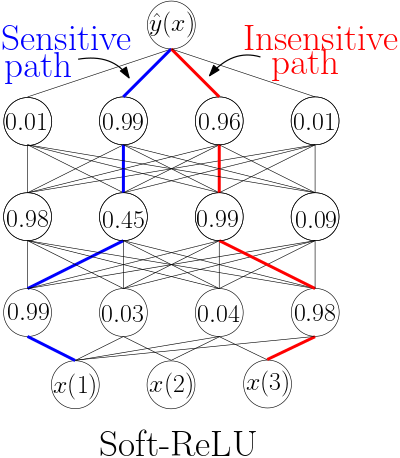
\includegraphics[scale=0.5]{figs/nnsoft.png}
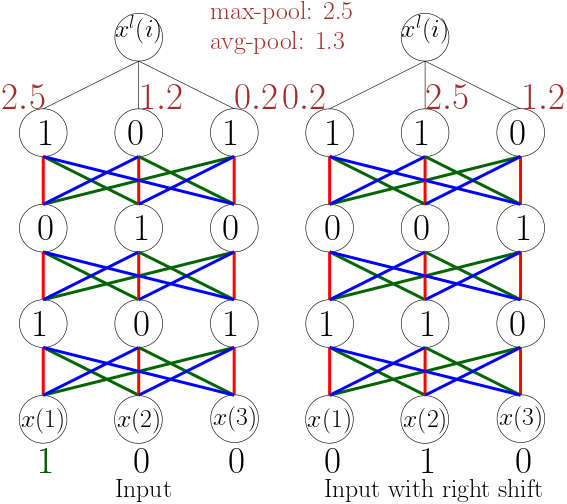
\includegraphics[scale=0.5]{figs/nnconv.png}
%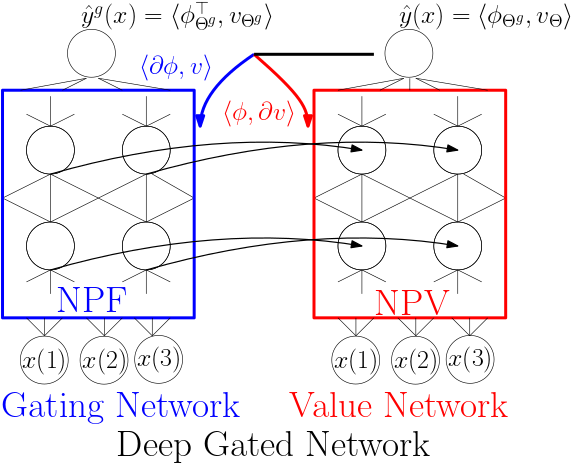
\includegraphics[scale=0.5]{figs/nntwin-blck.png}
%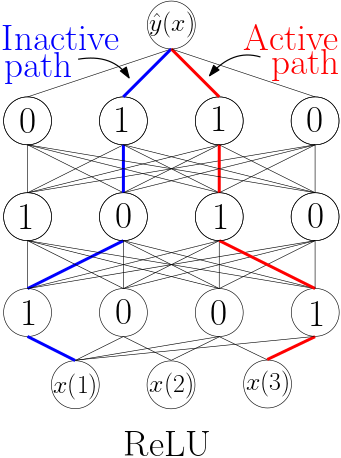
\includegraphics[scale=0.5]{figs/nn.png}
%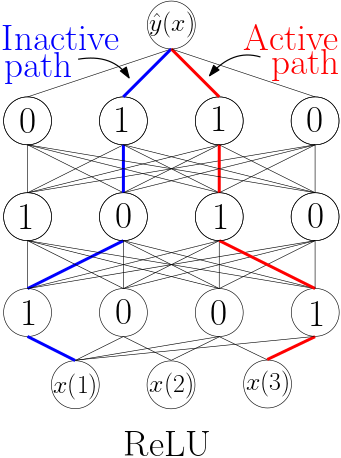
\includegraphics[scale=0.5]{figs/nn.png}
\end{tabular}
}
%\end{minipage}
%\begin{minipage}{0.18\columnwidth}
%\resizebox{\columnwidth}{!}{
%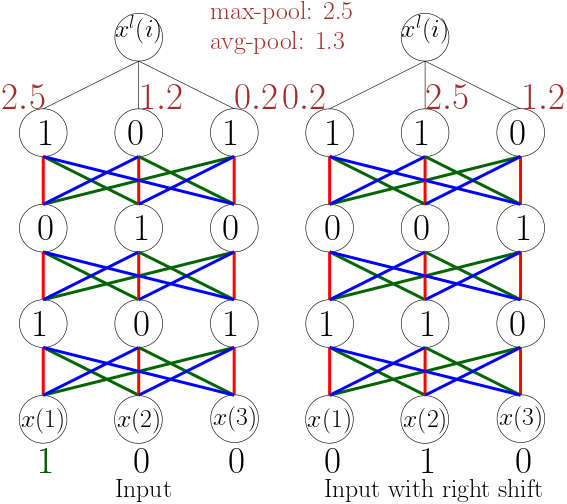
\includegraphics[scale=0.5]{figs/nnconv.png}
%}
%\end{minipage}
\caption{Cartoon illustration of usefulness of path-view and DGN framework.}
\label{fig:cartoon}
\end{figure*}
\subsection{Information Flow: First-Order}
$1.$ \textbf{Value Gradient} $\ip{\phi_{x,\Theta},\partial v_\Theta}$ (see \eqref{eq:zero}) flows through the active sub-network. To see this, $\ip{\phi_{x,\Theta},\partial v_{\Theta}}=\sum_{p\in[P]}x(\I_0(p))A_{\Theta}(x,p)\partial v$, i.e., only paths $p$ with $A_{\Theta}(x,p)=1$ contribute to the summation and $\partial v_{\Theta}(p)$ is non-zero only for those weights through which the path $p$ passes.\\
$2.$ \textbf{Feature Gradient}  $\ip{\partial\phi_{x,\Theta},v_{\Theta}}=\sum_{p\in [P]}x(\I(p)) \partial(A_{\Theta}(x,p)) v_{\Theta}(p)$. Note that, in the case of ReLU activations the gating values are either $0$ or $1$, and hence $\partial(A_{\Theta}(x,p))=0$. However, the gating values and hence the path activities $A_{\Theta_t}(\cdot,\cdot)$ changes during training. This artefact arising due to non-differentiability can be fixed by considering a \emph{soft-ReLU} activation. 
%where, for a pre-activation input $q\in\R$ the output is given by $q\frac{1}{1+\exp(-\beta q)}$ as opposed to $q\mathbbm{1}_{\{q>0\}}$ of the ReLU. 
Soft-ReLU `trick' enables us to capture the terms related to feature learning in our analysis. The difference between hard and soft gates can be seen cartoons $(a)/(b)$ and $(c)$ in \Cref{fig:cartoon}, where negative/positive values lead to $0/1$ in the case of hard gating, and close to $0/1$ in the case of soft-gating.\\
$3.$ \textbf{Sensitive Sub-Network:} In a DNN with soft-ReLU, $\partial A_{\Theta}(x,p)=\sum_{l=1}^d \partial G_{x,\Theta}(l)\Pi_{l'\neq l}G_{x,\Theta}(l')$ is significant for those paths $p$ for which one of the $d-1$ gating values is close to $0.5$ (say such a gate is in layer $l$, and for such a gate $\partial G_{x,\Theta}$ is significant) and rest of the $d-2$ gates are close to $1$, so that $\Pi_{l'\neq l}G_{x,\Theta}(l')$ is significant. The set of paths for which $\partial A_{\Theta}(x,p)$ is significant, form the sensitive sub-network for that input. The sensitive paths are shown in cartoon $(c)$ of \Cref{fig:cartoon}. In the case of, standard ReLU, sensitive paths are those which contain one of the gates with pre-activation close to $0$, and rest of the $d-2$ gates are $1$.
\begin{comment}
\subsection{Deep Gated Network (DGN)}
The NPFs are zeroth-order features stored solely in the gates of a DNN. In this paper, we separate out the NPFs from the NPVs. To this end, we introduce the deep gated network (DGN) framework, wherein, the output of a hidden unit is obtained as a product of its pre-activation and a gating value. A DGN has two network namely i) the gating network which holds the gating values and hence the NPF, and ii) a value network which holds the NPVs. %We denote a DNG by $\N(\Theta_t;\G(\Tg_t,\beta)$ or simply $\N(\Theta_t;\Tg_t,\beta)$
\begin{table}[h]
\begin{minipage}{0.5\columnwidth}
\resizebox{\columnwidth}{!}{
\begin{tabular}{|c|c|}\hline
Gating Network: $\G(\Tg_t,\beta)$\\\hline
$z_{x,\Tg_t}(0)=x$  \\\hline
$q_{x,\Tg_t}(l)={\Tg_t(l)}^\top z_{x,\Tg_t}(l-1)$ \\\hline
$z_{x,\Tg_t}(l)=q_{x,\Tg_t}(l)\odot G_{x,\Tg_t}(l)$ \\\hline
{$\begin{aligned}\beta >0: G_{x,\Tg_t}(l,i)&=\frac{1+\epsilon}{1+\exp(-\beta q_{x,\Tg_t}(l,i))} \\ \beta=\infty: G_{x,\Tg_t}(l,i)&=\mathbbm{1}_{\{q_{x,\Tg_t}(l,i)>0\}}\end{aligned}$}\\\hline 
\end{tabular}
}
\end{minipage}
\begin{minipage}{0.5\columnwidth}
\resizebox{\columnwidth}{!}{
\begin{tabular}{|l|l|}\hline
\multicolumn{2}{|c|}{Value Network: $\N(\Theta_t;\G_t)$}\\\hline 
Input layer & $z_{x,\Theta_t}(0)=x$ \\\hline
Pre-activation & $q_{x,\Theta_t}(l)={\Theta_t(l)}^\top z_{x,\Theta_t}(l-1)$\\\hline
Layer output & $z_{x,\Theta_t}(l)=q_{x,\Theta_t}(l)\odot G_{x,t}(l)$ \\\hline
Final output & $\hat{y}_t(x)={\Theta_t(d)}^\top z_{x,\Theta_t}(d-1)$\\\hline
Gating Values& $\begin{aligned}\G_t\stackrel{def}=\{G_{x_{s},t}(l,i), \forall s\in[n],\\l\in[d-1],i\in[w]\}\end{aligned}$\\\hline
\end{tabular}
}
\end{minipage}
\caption{$q(l),z(l)$ and $G(l)$ are $w$-dimensional quantities}
\label{tb:dgn}
\end{table}
\end{comment}